\begin{solution}
    I calculated the Variance Ratio statistic using up to 20 lags for both the value and the equal-weighted indices for the periods required and the results are shown on Figures~\ref{fig:vrtest_value_sample1}-\ref{fig:vrtest_equal_sample2}. \\
    Recall that the VR statistic can be written as a positive linear combination of the autocorrelation coefficients:
    \[
        VR\of{q} \approx 1 + 2\sum_{k=1}^{q-1} \bp{1-\frac{k}{q}} \rho_k
    \]
    Therefore we may interpret the direction of the autocorrelation (specially on \(q=2\) as the sign of the coefficient. \\
    For the value weighted portfolio, there is evidence pointing to the existence of \textbf{negative} autocorrelation for the sample of 2007-2022 only. The results are significant up until \(q = 11\) when using the HLZ std. dev. and \(q=8\) when using the LM std. dev. as seen on Figure~\ref{fig:vrtest_value_sample2}. For the sample of 1991-2006, there is no evidence of autocorrelation. \\
    The results are different for the equal-weighted portfolio. As we can see in Figures~\ref{fig:vrtest_equal_sample1} and \ref{fig:vrtest_equal_sample2}, the period between 1991 and 2006 shows strong signs of positive autocorrelation. The results are significant for the 20 values of \(q\) that were tested and the Variance Ratio statistic is always increasing, indicating that each one of the autocorrelations may be positive. For the sample of 2007-2022, the results are not significant for any of the values of \(q\) tested. All these results are consistent with either the HLZ or the LM std. deviations.\\
    \begin{figure}[!htbp]
        \centering
        \caption{Variance Ratio Test for the Value Weighted Index for 1991-2006}
        \label{fig:vrtest_value_sample1}
        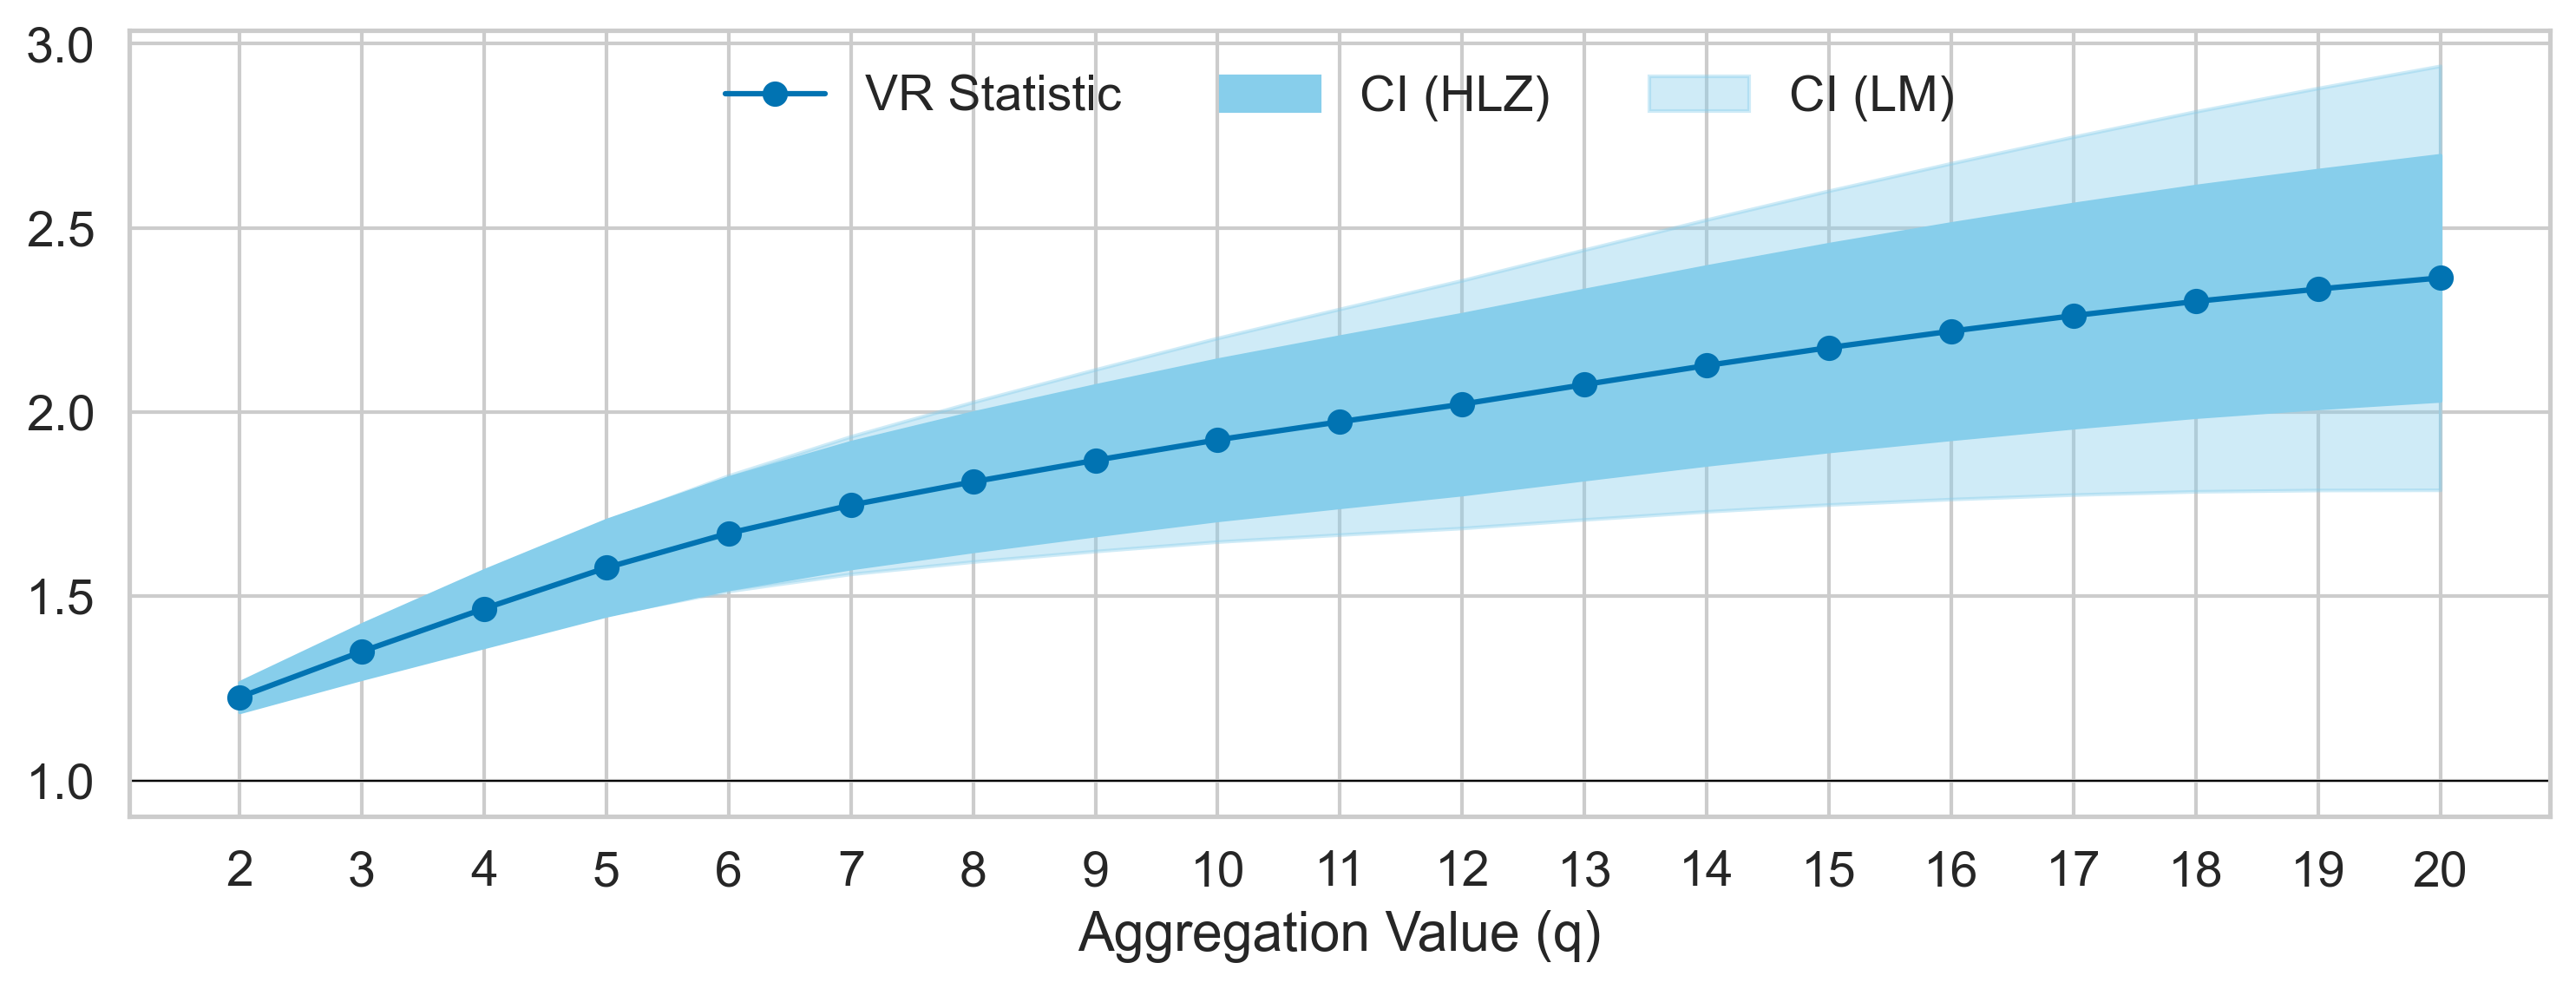
\includegraphics[width=1\textwidth]{vrtest_equal_sample1.png}
    \end{figure}
    \begin{figure}[!htbp]
        \centering
        \caption{Variance Ratio Test for the Value Weighted Index for 2007-}
        \label{fig:vrtest_value_sample2}
        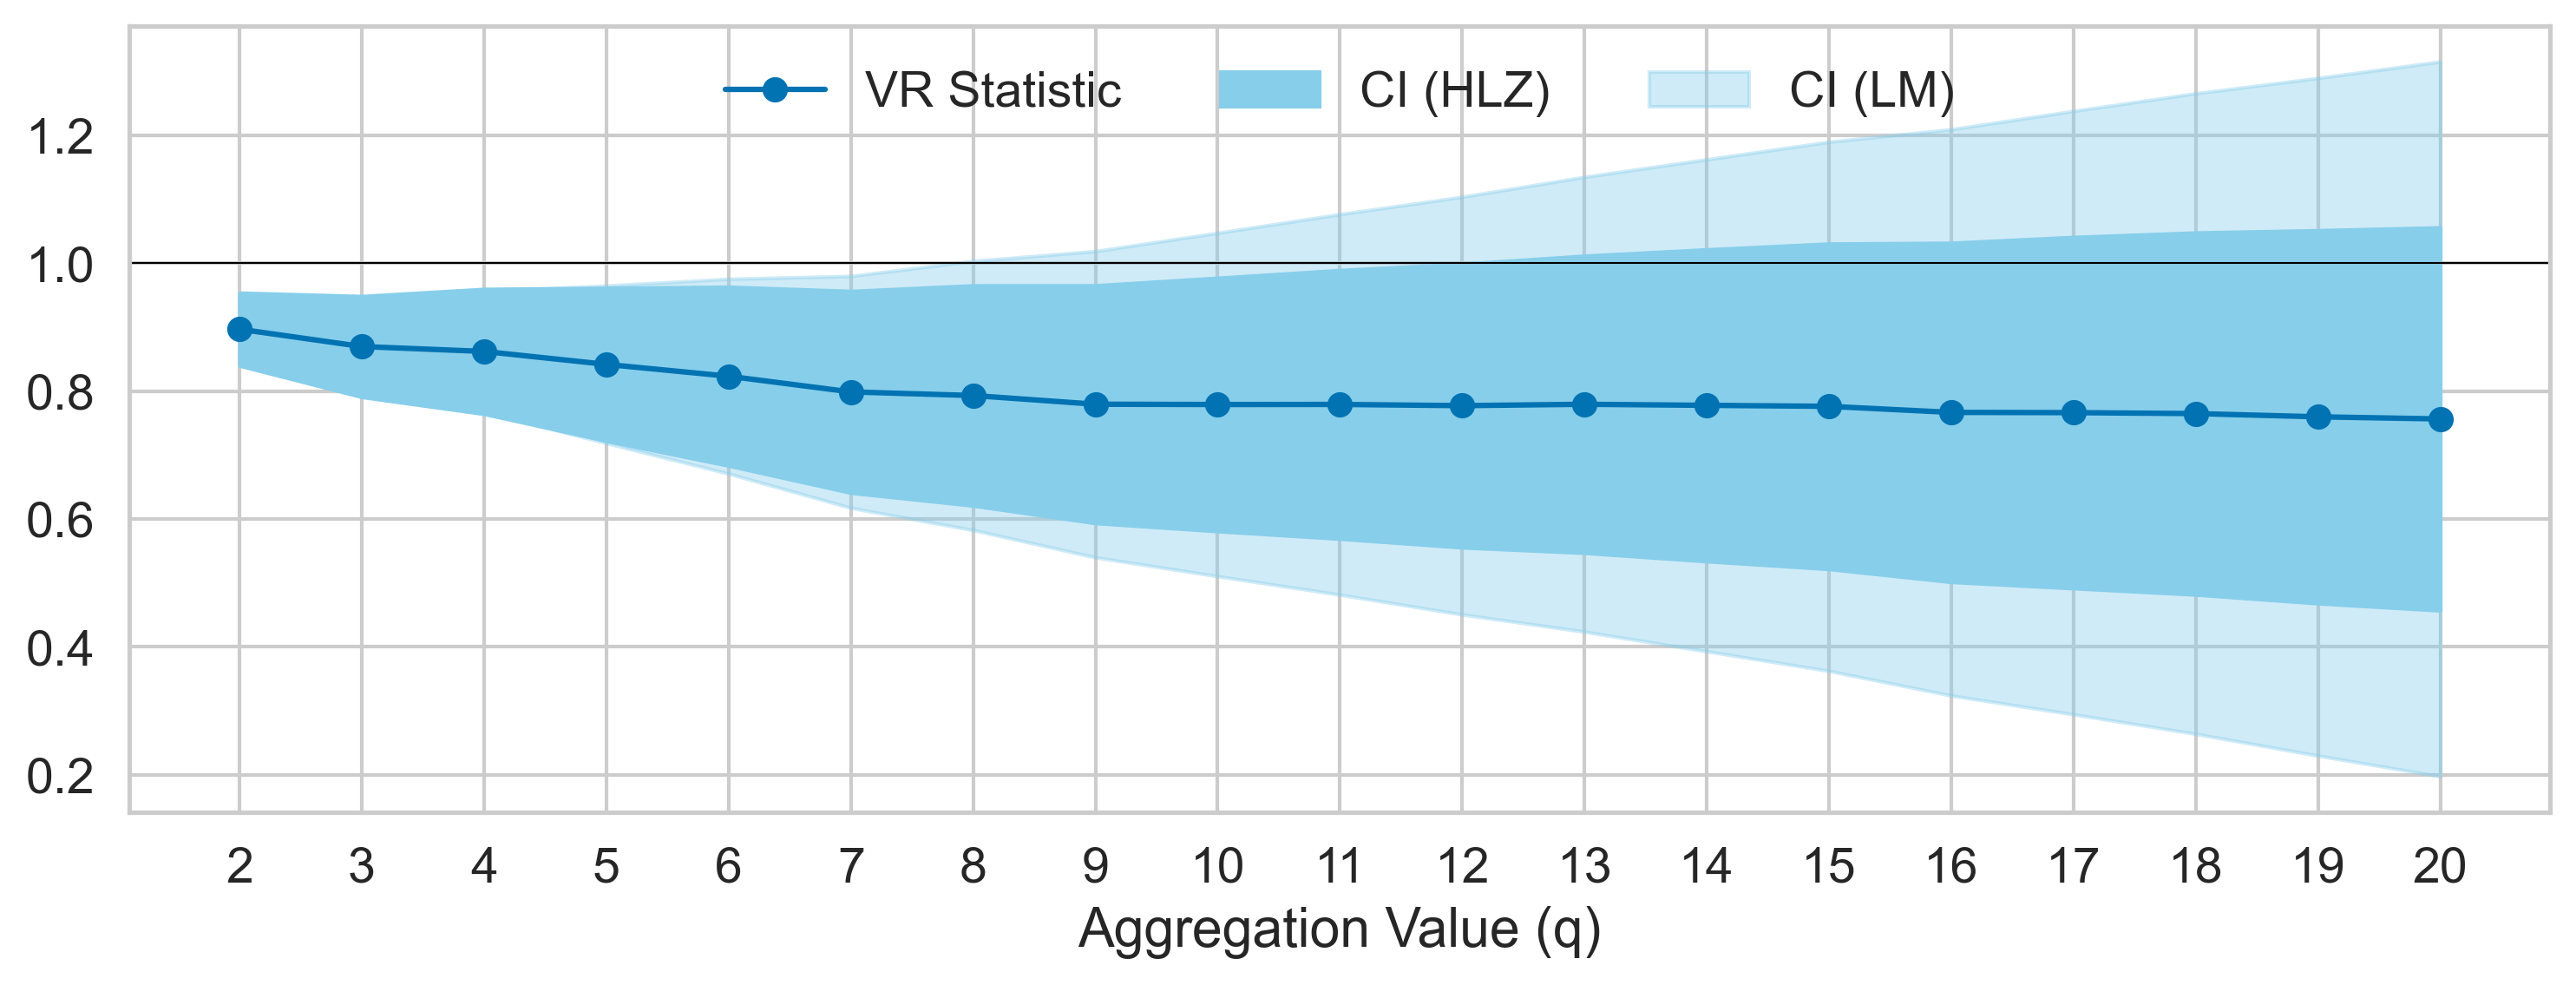
\includegraphics[width=1\textwidth]{vrtest_value_sample2.png}
    \end{figure}
    \begin{figure}[!htbp]
        \centering
        \caption{Variance Ratio Test for the Equal Weighted Index for 1991-2006}
        \label{fig:vrtest_equal_sample1}
        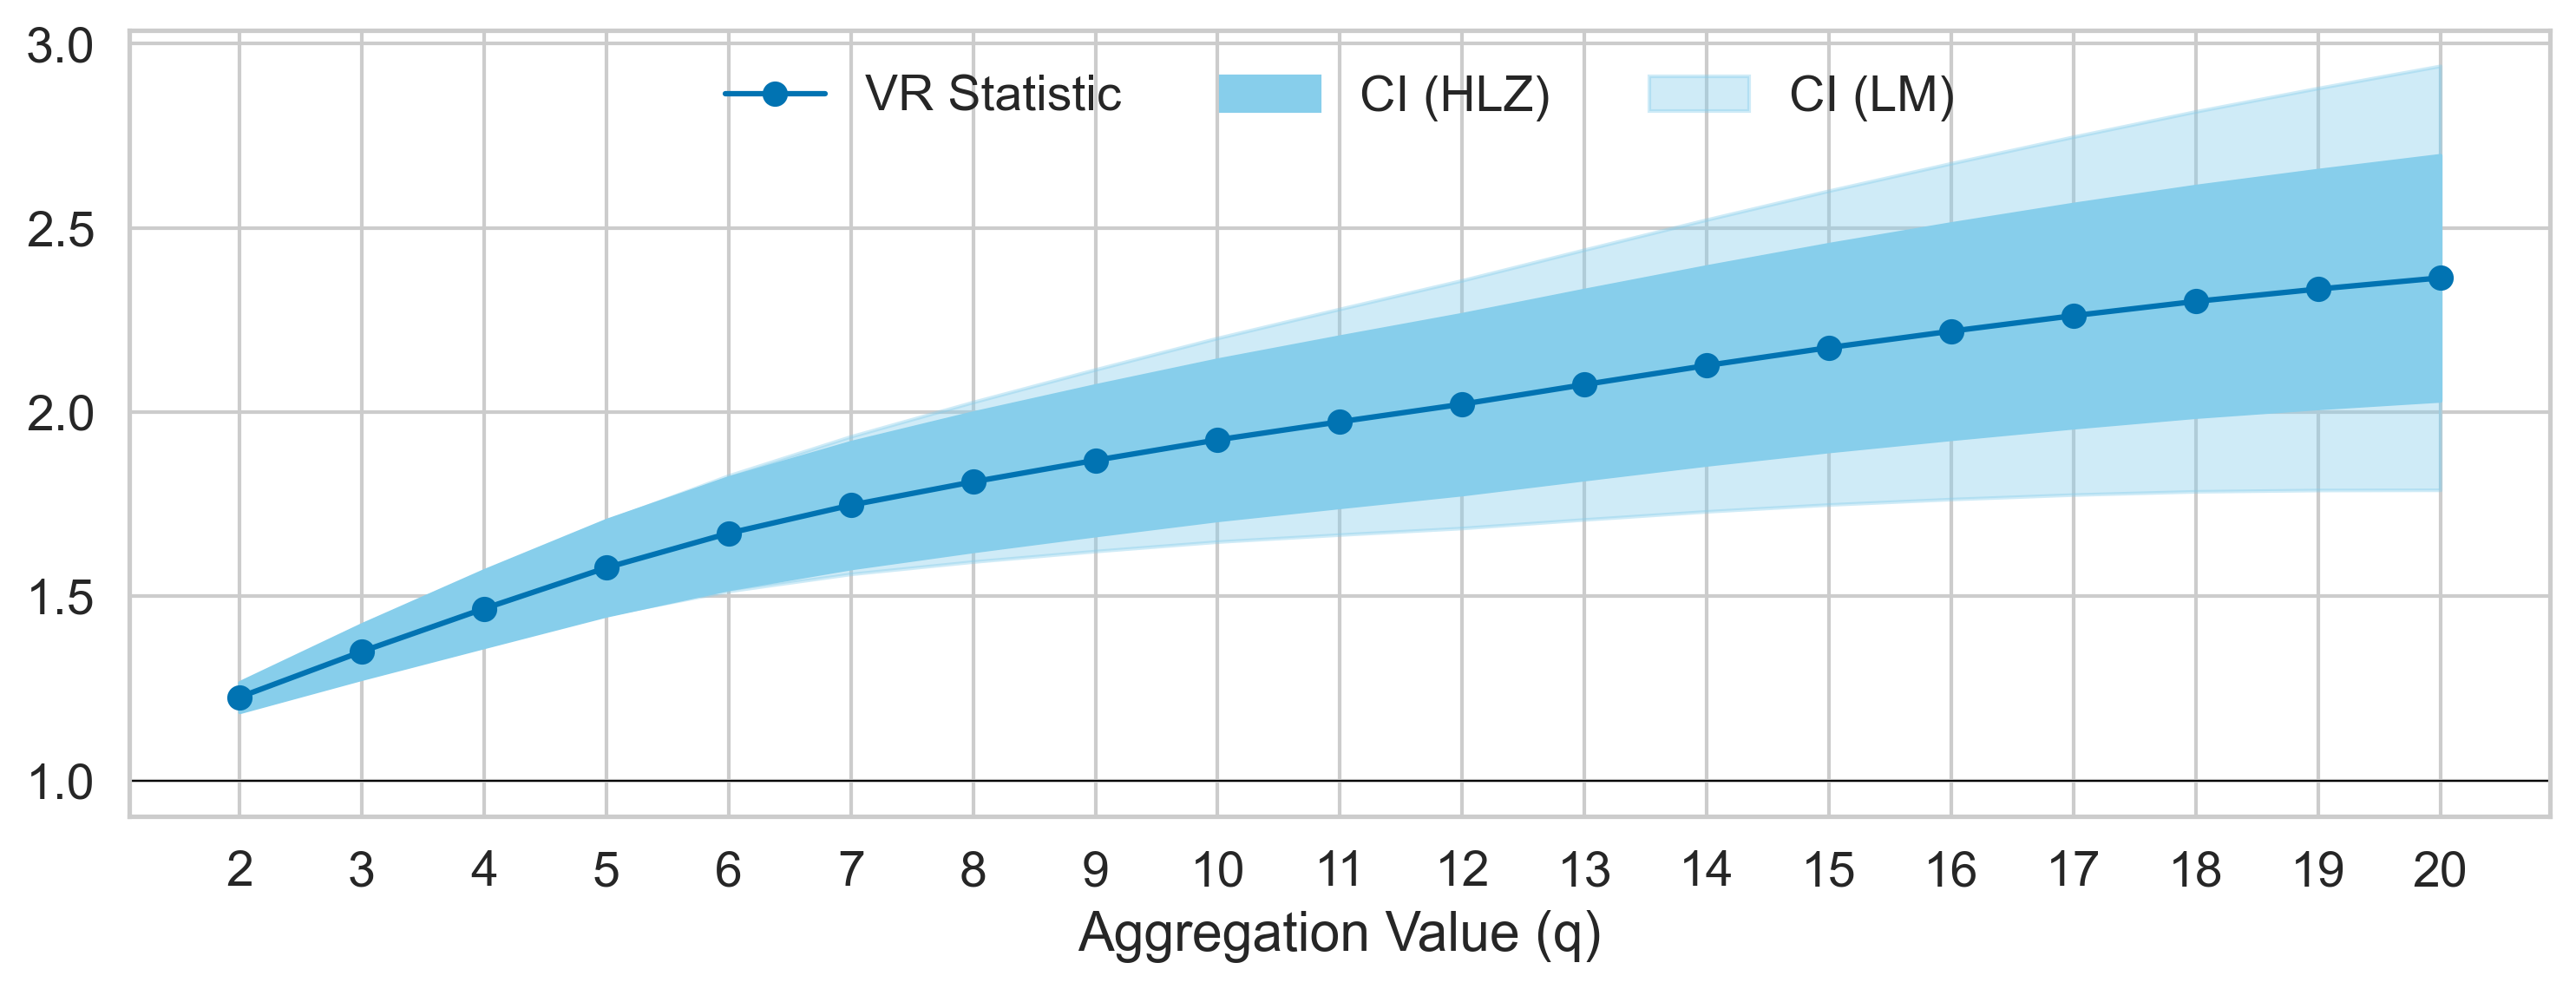
\includegraphics[width=1\textwidth]{vrtest_equal_sample1.png}
    \end{figure}
    \begin{figure}[!htbp]
        \centering
        \caption{Variance Ratio Test for the Equal Weighted Index for 2007-}
        \label{fig:vrtest_equal_sample2}
        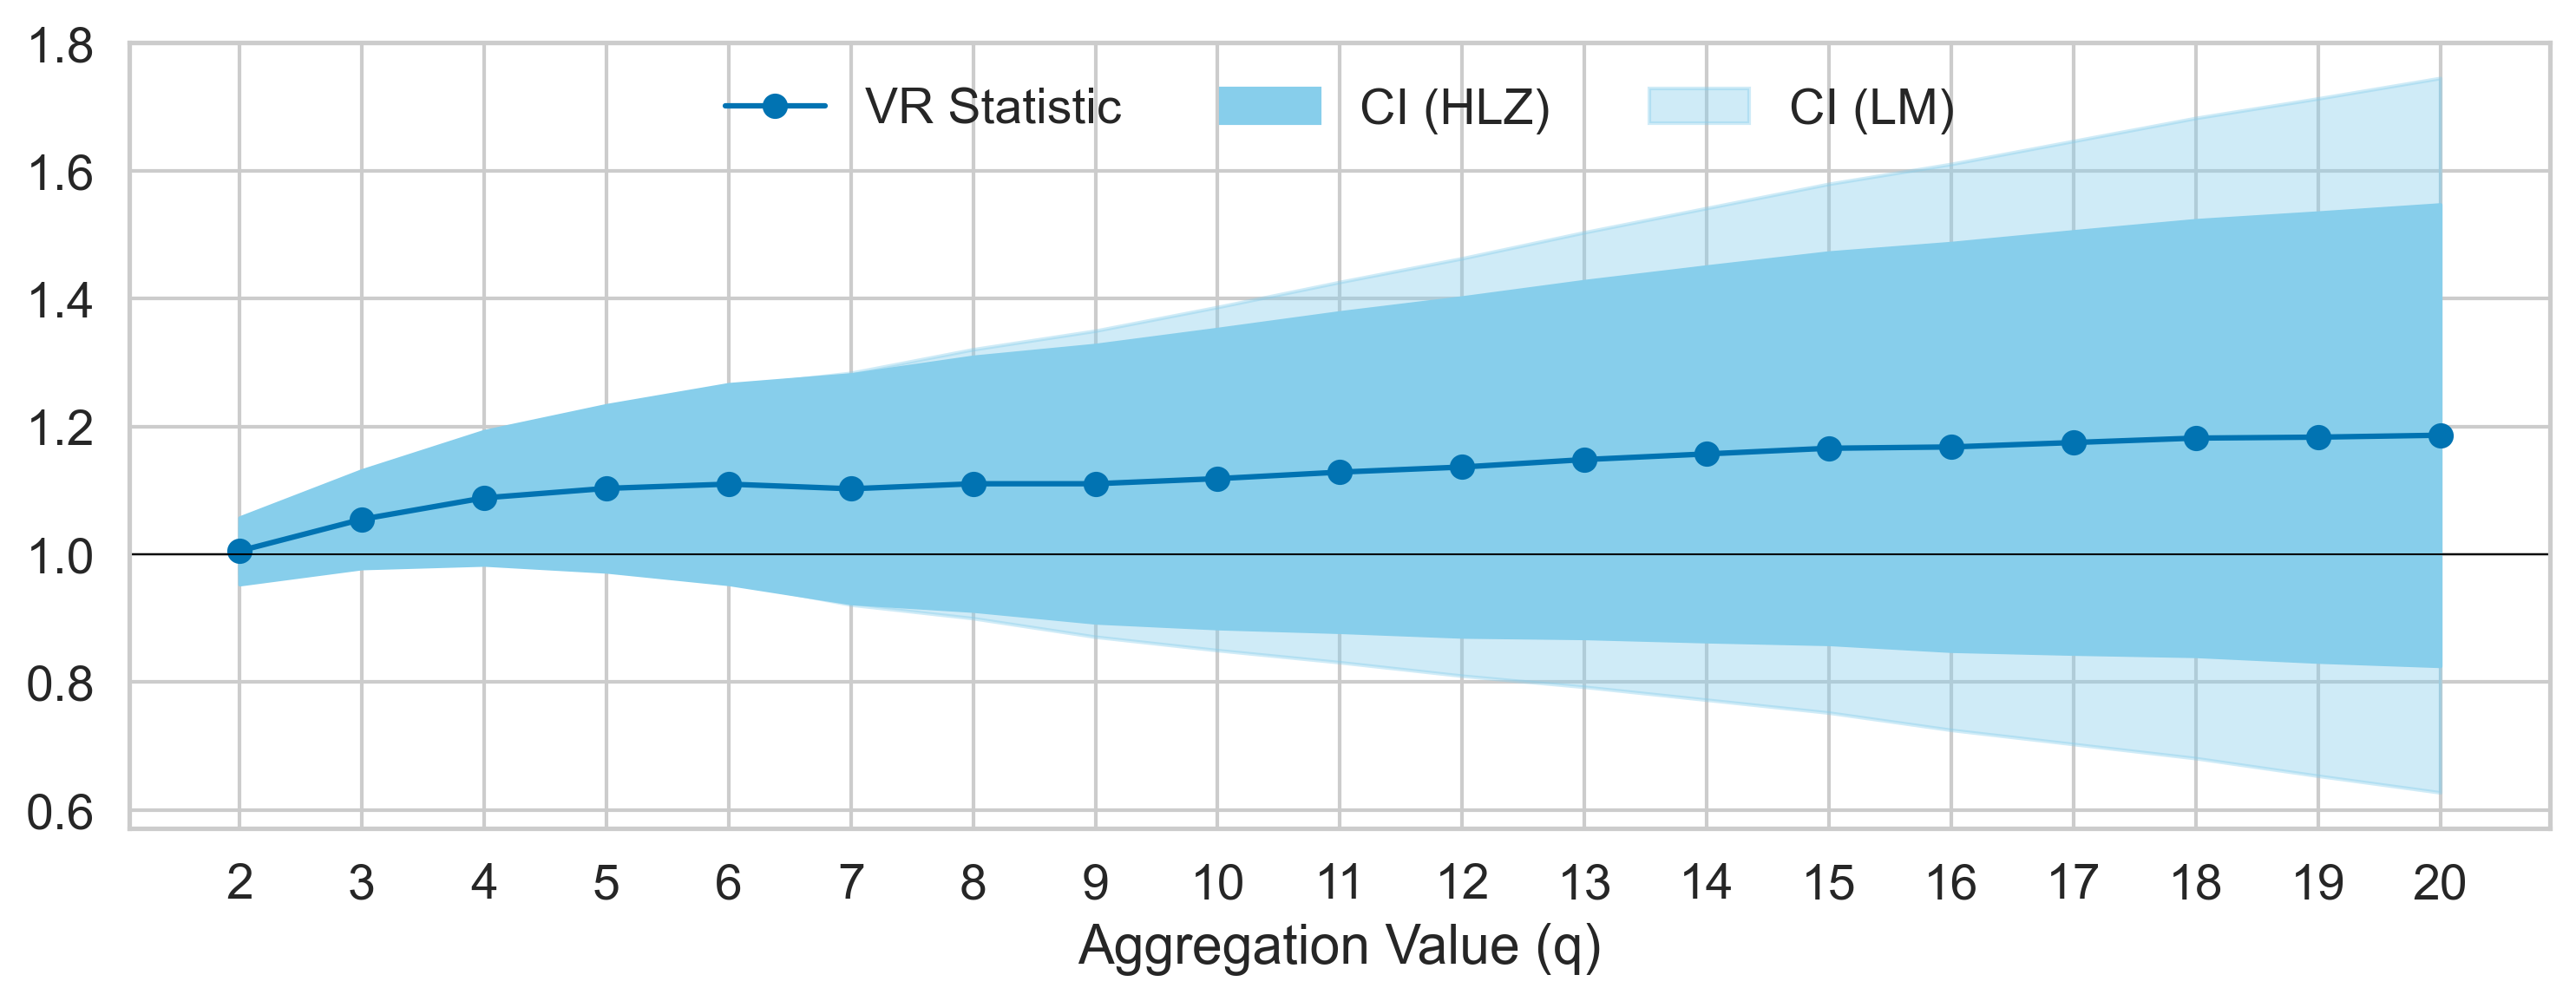
\includegraphics[width=1\textwidth]{vrtest_equal_sample2.png}
    \end{figure}
\end{solution} 
